\chapter{今後の展望}
\label{chp:first}

\section{段落と改行}
\label{sec:paragraph}

段落頭の字下げは自動で行われるため、全角スペースによる手動調整は不要であり、禁止である。
\LaTeX ソース中での改行は空行を挟まない場合は無視される。
ソース内では自分で編集しやすいように改行してよい。

このように、空行を挟むと改段落となる。
また、強制改行は\\このように \verb+\\+ で強制的に行うことができる。
しかし、この場合は段落の字下げもされないため、改段落を行う用途には空行を用いるべきで、
強制改行(\verb+\\+)は利用すべきではない。

しかしながら、例えば \verb+\verb+ 環境やインライン数式を用いる場合などで、
\verb+abcdefghijklmnopqrstuvwxyzABCDEFGHIJKLMNOPQRSTUVWXYZ+ 
というようにページ幅を超えてしまったり、前の行が間延びしてしまうようなケースがある。
そのような場合、\verb+\\+ を用いて強制改行により \\
\verb+abcdefghijklmnopqrstuvwxyzABCDEFGHIJKLMNOPQRSTUVWXYZ+ 
というように用いるとよい。

\section{箇条書き}
\label{sec:enum}

数字を使った場合の箇条書きの例を示す。

\begin{enumerate}
 \item 数字の付いた箇条書きの例
 \item こんな感じで手順などを列挙
\end{enumerate}

数字を付けずに列挙したい場合は itemize 環境を使う。
このようにあるキーワードを指定して \verb+\begin(}+ と \verb+\end{}+ で
囲む範囲のことを○○環境と呼ぶ。

\begin{itemize}
 \item 順番などを伴わない箇条書きの例
 \item 材料や要素を純粋に列挙したい場合に使用
\end{itemize}

enumerate 環境や itemize 環境は、入れ子構造を持つことができる。
例えば enumerate 環境の場合、以下のようになる。
\begin{enumerate}
 \item 東京都
 \begin{enumerate}
  \item 八王子市
  \item 多摩市
 \end{enumerate}
 \item 神奈川県
 \begin{enumerate}
  \item 横浜市
  \item 川崎市
 \end{enumerate}
 \item 山梨県
\end{enumerate}

\section{図表と参照}
\label{sec:fig_tbl}

図を挿入する際は以下のように書く。
必ずキャプションを付けるとともに、図に対する説明を本文中で記載すること。
何かの手違いで図が表示されなくなったとしても、文章で意味が通じるくらいに説明するのを目安にすること。
以下の図 \ref{fig:sample} と図 \ref{fig:ferret} は、適当なサンプル画像である。

\begin{figure}[H]
  \centering
  
\includegraphics[width=6.4cm]{./fig/fig-sample.eps}
  \caption{適当なサンプル}
% \url{http://www.this.is.sample.url/} % Web上のデータの場合、参照先URLを明記
  \label{fig:sample}
\end{figure}

\begin{figure}[H]
  \centering
  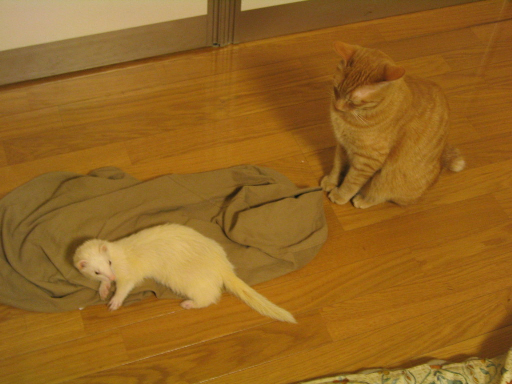
\includegraphics[width=6.4truecm]{./fig/ferret.png}
  \caption{適当なサンプル2}
% \url{http://www.this.is.sample.url/} % Web上のデータの場合、参照先URLを明記
  \label{fig:ferret}
\end{figure}

これまで、\LaTeX での図は伝統的には EPS 形式が用いられてきたが、
近年では JPEG 形式や PNG 形式など多くの画像フォーマットに対応している。
Inkscape や Illustrator 等のように直接 EPS 形式を出力する場合は EPS を用いることが望ましいが、
それ以外の状況では EPS への変換は行わずに画像ファイルを直接指定した方が品質が良い。
ただし、JPEG や PNG などの画像ファイルは EPS に比べて \LaTeX のコンパイルが長時間になる傾向があり、
あまり巨大な画像データを使用するとかなりコンパイル時間が長くなってしまうので、注意が必要である。
また、使用する画像ファイルはこのテンプレートのように
fig サブフォルダ内に格納することを推奨する。

図への参照は \verb+\label+ コマンドを用いて各図のキャプションにキーワードを付けておき、
文中で \verb+\ref+ コマンドによってキーワードを指定することで記述する。
キーワードは参照対象に応じてプリフィクスを付けることが望ましい。
以下の表 \ref{tbl:pre_list} に一般的に用いる参照対象ごとのプリフィクスを挙げる。

\begin{table}[H]
  \caption{ラベルに指定するキーワードのプリフィクス一覧}
  \label{tbl:pre_list}
  \centering
  \begin{tabular}{|l|l|r|} \hline
   参照対象	& プリフィクス \\ \hline
   章		& chp: \\ \hline
   節		& sec: \\ \hline
   図		& fig: \\ \hline
   表 		& tbl: \\ \hline
   式   	& eqn: \\ \hline
  \end{tabular}
\end{table}
手作業でのナンバリングは非効率極まりない上に必ずミスが出るので行わないこと。

\section{\LaTeX のコンパイル}
\LaTeX のコンパイルは、「コマンドプロンプト」や「PowerShell」などのコマンドライン上で「
latexmk」コマンドを用いる。
例えば、「M01xxyyy.tex」というファイルから PDF を作成したい場合は
\begin{verbatim}
    latexmk M01xxyyy
\end{verbatim}
というように、拡張子を抜いてコマンドラインで指定する。

また、コマンドラインに不慣れな学生は、
Atom エディタ等の \LaTeX パッケージを用いることも良案である。
Atom エディタを用いた \LaTeX の記述については、研究室 Wiki を参照のこと。
